\documentclass{article}

% packages
\usepackage{amsmath, amsthm, thmtools, amsfonts, amssymb, luacode, catchfile, tikzducks, hyperref, ifthen}
\ifcsname c@kobocompile\endcsname
	\usepackage[a5paper, total={1072pt, 1448pt}, margin=10pt, includeheadfoot]{geometry} % set page margins
\else
	\usepackage[a4paper, margin=50pt, includeheadfoot]{geometry}
\fi
\usepackage[shortlabels]{enumitem}
\usepackage[skip=3pt, indent=0pt]{parskip}

% language
\usepackage[bidi=basic, layout=tabular, provide=*]{babel}
\ifcsname c@english\endcsname
	\babelprovide[main, import]{english}
\else
	\babelprovide[main, import]{hebrew}
	\babelprovide{rl}
\fi
%\babelfont{rm}{Libertinus Serif}
\babelfont{rm}[Renderer=Harfbuzz]{Libertinus Serif}
\babelfont{sf}{Libertinus Sans}
\babelfont{tt}{Libertinus Mono}

% style
\AddToHook{cmd/section/before}{\clearpage}	% Add line break before section
\linespread{1.3}
\setcounter{secnumdepth}{0}		% Remove default number tags from sections, this won't do well with theorems
\AtBeginDocument{\setlength{\belowdisplayskip}{3pt}}
\AtBeginDocument{\setlength{\abovedisplayskip}{3pt}}
\graphicspath{ {../images/} }

% operators
\DeclareMathOperator\cis{cis}
\DeclareMathOperator\Sp{Sp}
\DeclareMathOperator\tr{tr}
\DeclareMathOperator\im{Im}
\DeclareMathOperator\re{Re}
\DeclareMathOperator\diag{diag}
\DeclareMathOperator*\lowlim{\underline{lim}}
\DeclareMathOperator*\uplim{\overline{lim}}
\DeclareMathOperator\rng{rng}
\DeclareMathOperator\Sym{Sym}
\DeclareMathOperator\Arg{Arg}
\DeclareMathOperator\Log{Log}
\DeclareMathOperator\dom{dom}
\DeclareMathOperator\supp{Supp}
\DeclareMathOperator\var{Var}
\DeclareMathOperator\cov{Cov}

% commands
%\renewcommand\qedsymbol{\textbf{מש''ל}}
%\renewcommand\qedsymbol{\fbox{\emoji{lizard}}}
\newcommand{\Aa}[0]{\mathcal{A}}
\newcommand{\Bb}[0]{\mathcal{B}}
\newcommand{\CC}[0]{\mathbb{C}}
\newcommand{\Cc}[0]{\mathcal{C}}
\newcommand{\EE}[0]{\mathbb{E}}
\newcommand{\FF}[0]{\mathbb{F}}
\newcommand{\Ff}[0]{\mathcal{F}}
\newcommand{\Ii}[0]{\mathcal{I}}
\newcommand{\Gg}[0]{\mathcal{G}}
\newcommand{\Ll}[0]{\mathcal{L}}
\newcommand{\Mm}[0]{\mathcal{M}}
\newcommand{\NN}[0]{\mathbb{N}}
\newcommand{\Nn}[0]{\mathcal{N}}
\newcommand{\PP}[0]{\mathbb{P}}
\newcommand{\Pp}[0]{\mathcal{P}}
\newcommand{\QQ}[0]{\mathbb{Q}}
\newcommand{\RR}[0]{\mathbb{R}}
\newcommand{\Rr}[0]{\mathcal{R}}
\newcommand{\Ss}[0]{\mathcal{S}}
\newcommand{\TT}[0]{\mathbb{T}}
\newcommand{\Uu}[0]{\mathcal{U}}
\newcommand{\Vv}[0]{\mathcal{V}}
\newcommand{\Ww}[0]{\mathcal{W}}
\newcommand{\ZZ}[0]{\mathbb{Z}}
\newcommand{\acts}[0]{\circlearrowright}
\newcommand{\explain}[2] {
	\begin{flalign*}
		 && \text{#2} && \text{#1}
	\end{flalign*}
}
\newcommand{\maketitleprint}[0]{ \begin{center}
	%\begin{tikzpicture}[scale=3]
	%	\duck[graduate=gray!20!black, tassel=red!70!black]
	%\end{tikzpicture}	
	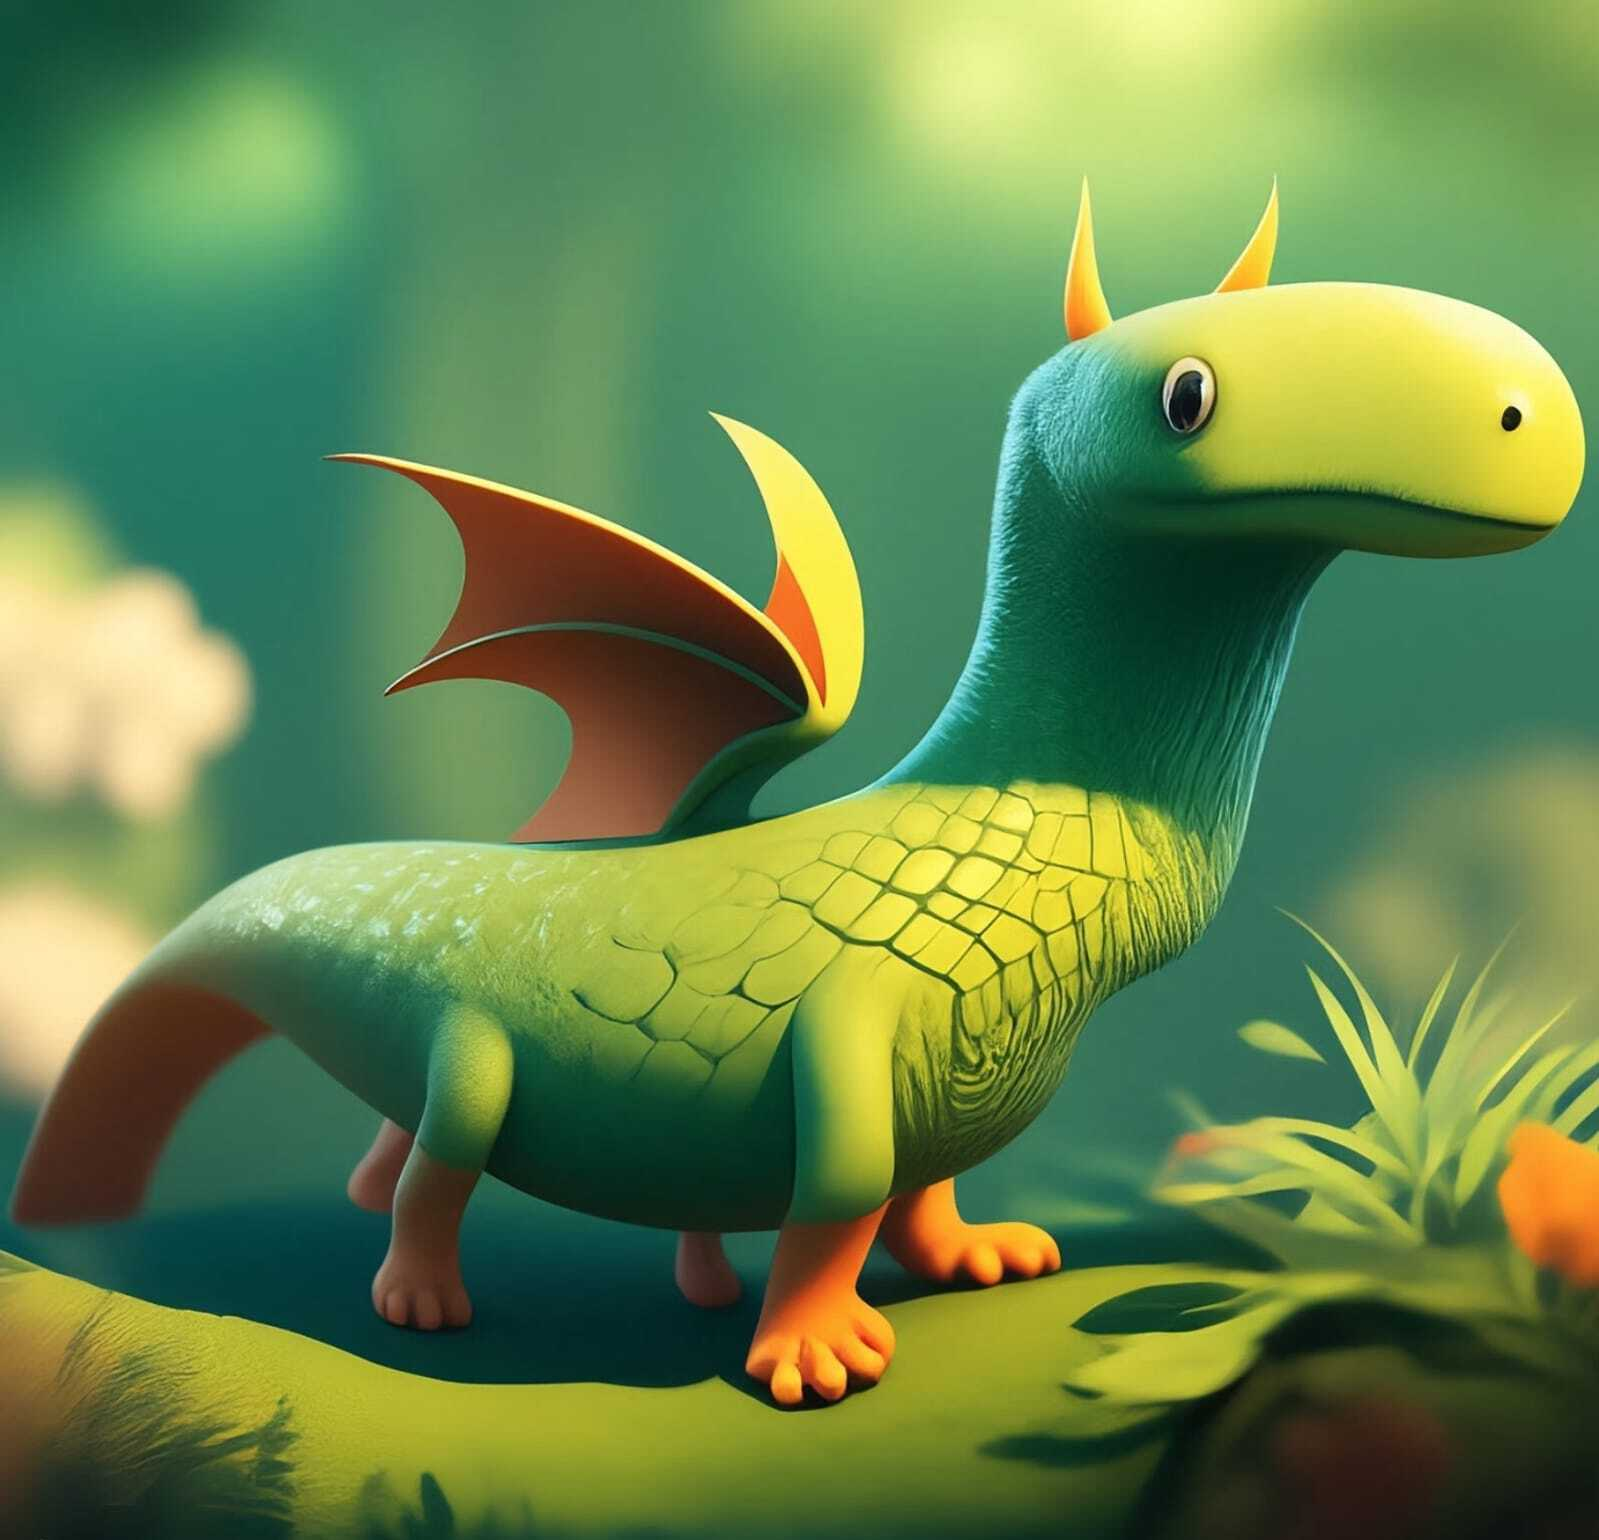
\includegraphics[width=6cm]{cover}
\end{center}
}

% theorem commands
\newtheoremstyle{c_remark}
	{}	% Space above
	{}	% Space below
	{}% Body font
	{}	% Indent amount
	{\bfseries}	% Theorem head font
	{}	% Punctuation after theorem head
	{.5em}	% Space after theorem head
	{\thmname{#1}\thmnumber{ #2}\thmnote{ \normalfont{\text{(#3)}}}}	% head content
\newtheoremstyle{c_definition}
	{3pt}	% Space above
	{3pt}	% Space below
	{}% Body font
	{}	% Indent amount
	{\bfseries}	% Theorem head font
	{}	% Punctuation after theorem head
	{.5em}	% Space after theorem head
	{\thmname{#1}\thmnumber{ #2}\thmnote{ \normalfont{\text{(#3)}}}}	% head content
\newtheoremstyle{c_plain}
	{3pt}	% Space above
	{3pt}	% Space below
	{\itshape}% Body font
	{}	% Indent amount
	{\bfseries}	% Theorem head font
	{}	% Punctuation after theorem head
	{.5em}	% Space after theorem head
	{\thmname{#1}\thmnumber{ #2}\thmnote{ \text{(#3)}}}	% head content

\ifcsname c@english\endcsname
	\theoremstyle{plain}
	\newtheorem{theorem}{Theorem}[section]
	\newtheorem{lemma}[theorem]{Lemma}
	\newtheorem{proposition}[theorem]{Proposition}
	\newtheorem*{proposition*}{Proposition}
	%\newtheorem{corollary}[theorem]{אין חלופה עברית}

	\theoremstyle{definition}
	\newtheorem{definition}[theorem]{Definition}
	\newtheorem*{definition*}{Definition}
	\newtheorem{example}{Example}[section]
	\newtheorem{exercise}{Exercise}[section]

	\theoremstyle{remark}
	\newtheorem*{remark}{Remark}
	\newtheorem*{solution}{Solution}
	\newtheorem{conclusion}[theorem]{Conclusion}
	\newtheorem{notation}[theorem]{Notation}
\else
	\theoremstyle{c_plain}
	\newtheorem{theorem}{משפט}[section]
	\newtheorem{lemma}[theorem]{למה}
	\newtheorem{proposition}[theorem]{טענה}
	\newtheorem*{proposition*}{טענה}
	%\newtheorem{corollary}[theorem]{אין חלופה עברית}

	\theoremstyle{c_definition}
	\newtheorem{definition}[theorem]{הגדרה}
	\newtheorem*{definition*}{הגדרה}
	\newtheorem{example}{דוגמה}[section]
	\newtheorem{exercise}{תרגיל}[section]

	\theoremstyle{c_remark}
	\newtheorem*{remark}{הערה}
	\newtheorem*{solution}{פתרון}
	\newtheorem{conclusion}[theorem]{מסקנה}
	\newtheorem{notation}[theorem]{סימון}
\fi

% Questions related commands
\newcounter{question}
\setcounter{question}{1}
\newcounter{sub_question}
\setcounter{sub_question}{1}

\ifcsname c@english\endcsname
	\newcommand{\question}[1][0]{
		\ifthenelse{#1 = 0}{}{\setcounter{question}{#1}}
		\section{Question \arabic{question}}
		\addtocounter{question}{1}
		\setcounter{sub_question}{1}
	}

	\newcommand{\subquestion}[1][0]{
		\ifthenelse{#1 = 0}{}{\setcounter{sub_question}{#1}}
		\subsection{Part \alph{sub_question}}
		\addtocounter{sub_question}{1}
	}
\else
	\newcommand{\question}[1][0]{
		\ifthenelse{#1 = 0}{}{\setcounter{question}{#1}}
		\section{שאלה \arabic{question}}
		\addtocounter{question}{1}
		\setcounter{sub_question}{1}
	}

	\newcommand{\subquestion}[1][0]{
		\ifthenelse{#1 = 0}{}{\setcounter{sub_question}{#1}}
		\subsection{סעיף \localecounter{letters.gershayim}{sub_question}}
		\addtocounter{sub_question}{1}
	}
\fi

% import lua and start of document
\directlua{common = require ('../common')}

\GetEnv{AUTHOR}

% headers
\author{\AUTHOR}
\date\today

\title{פתרון מטלה 01 --- מבוא לטופולוגיה, 80516}
% chktex-file 9
% chktex-file 17

\begin{document}
\maketitle
\maketitleprint{}

\question{}
יהי $(X, \tau)$ מרחב טופולוגי ותהי $A \subseteq X$ תת־קבוצה כלשהי. \\
נגדיר את טופולוגיית תת־המרחב על $X$ להיות $\tau \restriction A = \{ U \cap A \mid U \in \tau \}$.

\subquestion{}
נוכיח כי $\tau \restriction A$ היא טופולוגיה על $A$.
\begin{proof}
	נוכיח ישירות מהגדרת טופולוגיה. \\
	נבחין כי $X \in \tau$ ולכן $A = X \cap A \in \tau \restriction A$, ובאופן דומה גם $\emptyset \in \tau \restriction A$. \\
	נעבור לבדיקת סגירות על איחוד.
	תהי $I$ קבוצת אינדקסים ונניח ש־${\{ X_\alpha \}}_{\alpha \in I} \subseteq \tau \restriction A$, נניח גם שלכל $\alpha \in I$ קיים $X_\alpha \subseteq X_\alpha'$ כך ש־$X_\alpha' \in \tau$ (קיימים מהגדרה), אז,
	\[
		\bigcup_{\alpha \in I} X_\alpha
		= \bigcup_{\alpha \in I} X_\alpha' \cap A
		= \left( \bigcup_{\alpha \in I} X_\alpha' \right) \cap A
	\]
	אבל $\tau$ טופולוגיה ולכן סגורה לאיחוד ובהתאם $\bigcup_{\alpha \in I} X_\alpha' = Y \in \tau$ ולכן $Y \cap A \in \tau \restriction A$. \\
	נסיים ונבדוק סגירות סופית לחיתוכים, נניח ש־$X_i \in \tau \restriction A$ עבור $1 \le i \le n$ עבור $n \in \NN$ נתון.
	נניח גם ש־$X_i \subseteq X_i' \in \tau$ לכל $i$ מהצדקה זהה לזו בחלק הקודם.
	גם הפעם נובע,
	\[
		\bigcap_{i = 1}^n X_i
		= \bigcap_{i = 1}^n X_i' \cap A
		= \left( \bigcap_{i = 1}^n X_i' \right) \cap A
		\in \tau \restriction A
	\]
	ומצאנו משיקולים זהים יש סגירות סופית לחיתוך, ובהתאם $\tau \restriction A$ אכן טופולוגיה.
\end{proof}

\subquestion{}
נניח שקיימת מטריקה $\rho$ על $X$ כך ש־$\tau$ היא הטופולוגיה המושרית מ־$\rho$. \\
תהי $A \subset X$, נוכיח ש־ $\tau \restriction A$ מושרית מ־$(A, \rho \restriction A^2)$ כמרחב מטרי.
\begin{proof}
	נבחין כי מתקיים,
	\[
		x \in \tau \restriction A
		\iff \exists x' \in \tau, x = x' \cap A
	\]
	ונתון כי $\tau = \tau_\rho$, כלומר זוהי טופולוגיה מושרית ממטריקה $\rho$,
	ולכן $x'$ קבוצה פתוחה ב־$(X, \rho)$, לכן לכל $p \in x'$ קיים $r > 0$ כך ש־$B_r(p) \subseteq x'$.
	בהתאם לזה מתקיים גם $B_r(p) \cap A \subseteq x' \cap A = x$, אבל גם $B_r(p) \cap A = \{ z \in A \mid (\rho \restriction A^2)(p, z) < r \}$, כלומר הכדור נשאר פתוח ובהתאם $x$ קבוצה פתוחה במרחב המטרי המצומצם.
	מצאנו אם כן ש־$x \in \tau \restriction A$ אם ורק אם $x$ פתוחה ב־$(A, \rho \restriction A^2)$ ולכן $\tau \restriction A = \tau_{\rho \restriction A^2}$.
\end{proof}

\question{}
נמצא טופולוגיה על $\ZZ$ שבה אף נקודה אינה קבוצה פתוחה, אך הטופולוגיה המושרית על $\NN$ (בקורס זה ללא 0) היא הטופולוגיה הדיסקרטית.
\begin{solution}
	נגדיר את הבסיס $\Bb = \{-ZZ\} \cup \{ -\ZZ \cup \{ n \} \mid n \in \NN \}$, כלומר קבוצות מהצורה $\{ -1, -2, \dots \} \cup \{ n \}$ לכל $n$ טבעי, והקבוצה $\{-1, \dots\}$.
	נוודא שזהו אכן בסיס, לכל $z \in \ZZ$ או ש־$z \in \NN$ ואז $-ZZ \cup {z} \in \Bb$ או ש־$z < 0$ ולכן בהכרח קיימים איברים מכילים.
	בנוסף לכל $A, B \in \Bb$ מתקיים $A \ne B \implies A \cap B = -\ZZ$ ולכן נוכל לבחור כל איבר ב־$\Bb$ ולקבל שהתנאי השני לבסיס מתקיים.
	נגדיר $\tau = \tau_\Bb$, כלומר הטופולוגיה המושרית מהבסיס $\Bb$.

	נעבור לבדיקת תנאי התרגיל, אין אף נקודה שהיא קבוצה פתוחה, שכן כל איבר $x \in \tau_\Bb$ הוא איחוד של איברי $\Bb$, לכן בפרט $x \supseteq -\ZZ$ ואיננו יחידון. \\
	מהצד השני נבחן את $\tau \restriction \NN$, הפעם $\{ n \} \in \tau \restriction \NN$ לכל $n \in \NN$ ישירות מבדיקת הבסיס, ולכן זוהי הטופולוגיה הדיסקרטית.
\end{solution}

\subquestion{}
נמצא טופולוגיה על $\ZZ$ שבה אף נקודה אינה קבוצה פתוחה, אך לכל $n \ge 0$, הטופולוגיה המושרית על $[-n, n] \cap \ZZ$ היא הטופולוגיה הדיסקרטית.
\begin{solution}
	נגדיר את הבסיס $\Bb = \{ (\ZZ \setminus [-n, n]) \cup \{ k \} \mid n \in \NN, k \in \ZZ \cap [-n + 1, n - 1] \}$.
	נבחין כי לכל $m \in \ZZ$ אכן אפשר לבחור $ n = m + 1, k = m$, וכן לכל $A, B \in \Bb$,
	אם $m \in A \cap B$ אז או ש־$m$ גדול מ־$\max\{ n_A, n_B \}$ ונוכל לבחור קבוצה מתאימה, או ש־$k_A = k_B$ ו־$m = k_A$, אז נבחר $n = k + 1, k = k_A$.

	עתה משהוכחנו שזהו אכן בסיס, נבחן את הטופולוגיה $\tau_\Bb$, ברור כי אין יחידונים בטופולוגיה זו, זאת שכן נוכל לבחור $n \in \NN$ גדול מספיק כך שיופיע באיבר לכל איבר ב־$\tau_\Bb$.
	מן הצד השני, נקבע $n \in \NN$ ונבחן את $\tau_\Bb \restriction [-n, n]$, אז הקבוצות $((\ZZ \setminus [-n - 1, n + 1]) \cup \{k\}) \cap [-n, n] = \{ k \}$ נמצאת ב־$\tau_\Bb \restriction A$.
\end{solution}

\question{}
\subquestion{}
תהינה ${\{\tau_i\}}_{i \in I}$ טופולוגיות על קבוצה $X$. \\
נוכיח כי גם $\bigcap_{i \in I} \tau_i$ היא טופולוגיה על $X$.
\begin{proof}
	נוכיח את הטענה ישירות מהגדרת טופולוגיה. \\
	נבחין כי $\forall i \in I,\ X, \emptyset \in \tau_i$ מהגדרה, ולכן $X, \emptyset \in \bigcap_{i \in I} \tau_i$. \\
	נעבור לסגירות לאיחוד, נניח ש־$J$ קבוצת אינדקסים, ונניח כי $X_j \in \bigcap_{i \in I} \tau_i$ לכל $j \in J$.
	נניח גם ש־$X_j^i \in \tau_i$ כך ש־$X_j = \bigcap_{i \in I} \tau_i$, אז מתקיים,
	\[
		\bigcap_{j \in J} X_i
		= \bigcup_{j \in J} \bigcap_{i \in I} X_j^i
		= \bigcap_{i \in I} \bigcup_{j \in J} X_j^i
	\]
	אבל $\tau_i$ סגורה לאיחודים ולכן $\bigcup_{j \in J} X_j^i \in \tau_i$, ובהתאם קבוצה זו היא פתוחה ב־$\bigcap_{i \in I} \tau_i$. \\
	סגירות סופית לחיתוך זהה.
\end{proof}

\subquestion{}
נסיק שאם $P$ היא אוסף כלשהו של תתי־קבוצות של $X$ אז קיימת טופולוגיה מינימלית $\tau$ כך ש־$P \subset \tau$.
נקרא ל־$\tau$ טופולוגיה מינימלית המכילה את $P$.
\begin{proof}
	תהי $\Sigma = \{ \sigma \in \Pp(X) \mid P \subset \sigma, \sigma \text{ is a topology over } X \}$, נבחין כי זוהי אכן קבוצה מאקסיומת הפרדה (תכונות טופולוגיה הן מסדר ראשון), ולכן $\tau = \bigcap \Sigma$ טופולוגיה מסעיף א'.
	כמובן ש־$\tau$ מינימלית ביחס ההכלה מבין איברי $\Sigma$ ישירות מהגדרה.
\end{proof}

\subquestion{}
תהי $X = \{a, b, c\}$ ונגדיר $P = \{\{a\}, \{a, b\}, \{b, c\}\}$, נמצא את הטופולוגיה המינימלית המכילה את $P$.
\begin{solution}
	נניח ש־$\tau$ הטופולוגיה המקיימת זאת, אז בהכרח $P \subseteq \tau$, וכמובן $\emptyset, X \in \tau$.
	אנו יודעים ש־$\tau$ סגורה לחיתוכים (בקבוצה סופית כל חיתוך הוא סופי), לכן גם $\{b\} \in \tau$, והסגירות לאיחודים לא מוסיפה איברים לקבוצה, ולכן סיימנו.
\end{solution}

\question{}
יהיו $(X, \tau_X), (Y, \tau_Y)$ מרחבים טופולוגיים.

\subquestion{}
נגדיר טופולוגיה $\tau$ על $X \sqcup Y$ על־ידי $A \in \tau \iff \exists U \in \tau_X, V \in \tau_Y,\ A = U \sqcup V$. \\
נראה ש־$\tau$ היא טופולוגיה על $X \sqcup Y$.
\begin{proof}
	נבחין כי $\emptyset \in \tau_X, \tau_Y \implies \emptyset \in \tau$ וכן $X \in \tau_X, Y \in \tau_Y$ ולכן $A \in \tau$. \\
	נניח ש־$\{ X_i \} \subseteq \tau_X$ וש־$\{ Y_i \} \subseteq \tau_Y$ עבור $i \in I$ קבוצת אינדקסים כלשהי.
	מתקיים $X_i \sqcup Y_i \in \tau$ לכל $i \in I$, וכן מתקיים,
	\[
		\bigcup_{i \in I} X_i \sqcup Y_i
		= \left(\bigcup_{i \in I} X_i\right) \sqcup \left(\bigcup_{i \in I} Y_i\right)
	\]
	מתכונות איחוד זר, ונובע מהגדרת $\tau$ כי יש סגירות לאיחוד. \\
	נניח ש־$U, U' \in \tau_X, V, V' \in \tau_Y$, אז $(U \cap U') \sqcup (V \cap V') = (U \sqcup V) \cap (U' \sqcup V')$ ולכן נובע ש־$\tau$ סגורה גם לחיתוכים סופיים.
\end{proof}

\subquestion{}
נראה שהטופולוגיה $\tau$ המושרית על $X$ שווה ל־$\tau_X$ ושהטופולוגיה המושרית על $Y$ שווה ל־$\tau_Y$.
\begin{proof}
	מטעמי סימטריה מספיק להראות את נכונות הטענה על $X$ ו־$\tau_X$.
	\[
		U \in \tau_X
		\iff \exists V \in \tau_Y,\ U \sqcup V \in \tau
		\iff U \in \tau \restriction X
	\]
	כאשר הצעד הראשון נובע מהגדרת $\tau$ והצעד השני נובע מהגדרת הצמצום.
\end{proof}

\subquestion{}
תהיינה $X, Y$ קבוצות, נראה שכל טופולוגיה על $X \sqcup Y$ מתקבלת מטופולוגיה על $X$ וטופולוגיה על $Y$ באופן שתואר בסעיף א'.
\begin{proof}
	נניח ש־$\tau \subseteq \Pp(X \sqcup Y)$, ונוכיח שהיא שקולה לטופולוגיה המופיעה בסעיף א' עבור איזושהן טופולוגיות $\tau_X, \tau_Y$. \\
	נגדיר $\tau_X' = \tau \restriction X$, זהו צמצום של טופולוגיה ולכן בהכרח טופולוגיה, וכן $\tau_X'$ טופולוגיה מעל $X$, אבל אז מסעיף ב' נובע $\tau_X = \tau_X'$, נגדיר כך גם את $\tau_Y$ ומצאנו שאכן $\tau$ ניתנת לפירוק.
\end{proof}

\question{}
נראה ששני האוספים הבאים של קבוצות הם בסיסים לטופולוגיה כלשהי על $\RR$,
\[
	\Bb_1 = \{ [a, b) \mid a, b \in \RR \},
	\quad
	\Bb_2 = \{ [a, b) \mid a, b \in \QQ \}
\]
נראה גם כי שני הבסיסים לא יוצרים את אותה הטופולוגיה על $\RR$.
\begin{proof}
	נבדוק את התנאים לקיום בסיס עבור $\Bb_1$. \\
	נבחין כי $\bigcup \Bb_1 = \RR$, זאת שכן לכל $x \in \RR$ הקטע $[x, x + 1) \in \Bb_1$.
	נניח ש־$A, B \in \Bb_1$, וכן ש־$x \in A \cap B$, נבחין כי $A = [a, a'), B = [b, b')$ עבור ערכים כלשהם, ונבחר $c = \max\{a, b\}, c' = \min\{a', b'\}$, אז כמובן $C = [c, c') \in \Bb_1$ וכן $x \in C$,
	וגם $C = A \cap B$ ולכן בפרט $C \subseteq A \cap B$.

	עבור $\Bb_2$ ההוכחה זהה לחלוטין, זאת נוכל להסיק מצפיפות הרציונליים בממשיים.

	לבסוף נראה ש־$\tau_{\Bb_1} \ne \tau_{\Bb_2}$.
	נבחן את $[\sqrt{2}, 3) \in \tau_{\Bb_1}$ ונוכיח שאיבר זה לא נמצא ב־$\tau_{\Bb_2}$. \\
	אילו נניח בשלילה שהוא כן נמצא, אז נקבל שקיימת סדרת קטעים ${\{[a_i, b_i)\}}_{i \in I} \subseteq \Bb_2$ כך ש־$\bigcup_{i \in I} [a_i, b_i) = [\sqrt{2}, 3)$.
	בפרט נובע ש־$\inf \bigcup_{i \in I} [a_i, b_i) = \min_{i \in I} a_i = \sqrt{2}$, כאשר המינימום נובע מהסגירות המקומית של הקטעים, ולכן קיים $i \in I$ כך ש־$a_i = \sqrt{2}$, בסתירה ל־$a_i \in \QQ$ לכל $i \in I$.
\end{proof}

\end{document}
